\chapter{Research Proposal}
\label{ch:research_proposal}
To develop the parallel MCSA and FANM methods, a research plan is
proposed to drive their development and quantify their merits and
feasibility as compared to more conventional methods for linear and
nonlinear problems. We seek to rigorously verify both of these methods
and their implementation and will describe the means by which that
will be accomplished. Furthermore, the numerical experiments performed
will be constructed within a software framework that will permit an
agile development strategy. In this chapter we describe that
experimental framework and the progress achieved to date by its
use. In addition, we will a formulate a plan for verifying the new
Monte Carlo methods and prepare a set of numerical experiments that
will determine some of their properties. Finally, we select a
large-scale challenge problem designed to potentially demonstrate the
effectiveness of our new methods in the context of real-world,
production level applications for nuclear reactor analysis.

\section{Experimental Framework}
\label{sec:experimental_framework}
For all of our numerical experiments, we need to readily be able to do
two things: generate linear and nonlinear systems in parallel. To do
this effectively requires many software components to be implemented
including linear algebra data structures, a parallel communication
framework, mesh generation and partitioning, application of boundary
and initial conditions, automatic differentiation technology, and
other high-level framework technologies. These development of these
components, however, are not the focus of this work but rather the
necessary machinery needed for the experimental apparatus. We
therefore choose an environment in which all of these tools are
readily available in the form of production software implementations
and that will demonstrate scalability in high performance computing
environments. This environment will be based on the mathematical
framework of the finite element method and will permit an
algorithm-oriented design for the parallel stochastic solvers we will
develop.

\subsection{Finite Element Formulation}
\label{subsec:fem_assembly}
Choosing a finite element formulation for our physics problems permits
us flexibility from both a mathematical and software development
standpoint. We briefly review the \textit{finite element method} as
presented in Zienkiewicz's text \citep{zienkiewicz_finite_2005}. In
general, we are concerned with solving a set of differential
equations:
\begin{subequations}
  \begin{gather}
    \ve{A}(\ve{u}) = \ve{0},\ \forall \ve{u} \in \Omega \\
    \ve{B}(\ve{u}) = \ve{0},\ \forall \ve{u} \in \Gamma\:,
  \end{gather}
  \label{eq:finite_element_de}
\end{subequations}
where $\Omega$ is the domain over which the set of differential
equations is defined and $\Gamma$ is the boundary of that domain. We
then have a set of differential equations, $\ve{A}(\ve{u})$, in
residual form that represent the physics on the domain and the set
$\ve{B}(\ve{u})$ that is representative of those physics on the
boundary. As an alternative, we can instead state these differential
equations in an equivalent integral form via a conservation statement:
\begin{equation}
  \int_{\Omega} \ve{v}^T \ve{A}(\ve{u}) d\Omega + \int_{\Gamma}
  \bar{\ve{v}}^T \ve{B}(\ve{u}) d\Gamma = \ve{0} \:,
  \label{eq:fe_integral_form}
\end{equation}
where $\ve{v}$ and $\bar{\ve{v}}$ are arbitrary, finite-valued vectors
that satisfy the integral relation and the constraints in
Eq~(\ref{eq:finite_element_de}).

If the $n^{th}$-order derivative of $\ve{u}$ contains discontinuities
(i.e. is not smooth), then the integral form presented in
Eq~(\ref{eq:fe_integral_form}) is restricted in that only derivatives
up to order $n+1$ may appear in the functions $\ve{A}(\ve{u})$ and
$\ve{B}(\ve{u})$. We can relax this restriction by integrating
Eq~(\ref{eq:fe_integral_form}) by parts to arrive at the \textit{weak
  form} of the differential equations:
\begin{equation}
  \int_{\Omega} \ve{C}(\ve{v}^T) \ve{D}(\ve{u}) d\Omega +
  \int_{\Gamma} \ve{E}(\bar{\ve{v}}^T) \ve{F}(\ve{u}) d\Gamma = \ve{0}
  \:,
  \label{eq:fe_weak_form}
\end{equation}
where the new functional form now has lower-order derivatives in
$\ve{D}(\ve{u})$ and $\ve{F}(\ve{u})$, thus relaxing the smoothness
requirement.

In our experimental framework, we will formulate all of our problems
using the weak form of the differential equations as in
Eq~(\ref{eq:fe_weak_form}). Doing so allows us to leverage modern
finite element assembly engine software with embedded automatic
differentiation technology. Using the Panzer library in the Trilinos
scientific computing framework
\citep{notz_graph-based_2010,heroux_overview_2005}, function
evaluation routines in the form of Eq~(\ref{eq:fe_weak_form}) are
generated to represent the finite element problem and boundary
conditions. Per Bartlett's automatic differentiation work and an
associated parallel linear algebra framework, the equation sets for
all physics implemented are assembled into the nonlinear system. By
leveraging the general linear algebra framework, we are able to
abstract away those concepts in the Monte Carlo solvers implementation
and instead focus on an algorithm-oriented approach for the solver
implementation \citep{musser_algorithm-oriented_1994}.

\section{Progress to Date}
\label{sec:progress}
To date, progress has been made on development of the experimental
framework based on the Panzer library. Using this framework, several
preliminary objectives have been achieved including an implementation
of the MCSA algorithm using a general linear algebra framework and
initial analysis of its performance using both the direct and adjoint
Neumann-Ulam methods. Here we report the results of this work and its
relationship with future work.

\subsection{Generalization of MCSA for Linear Problems}
\label{subsec:mcsa_generalization}
Previous implementations of MCSA had an entirely physics-based
approach \citep{evans_monte_2009,evans_monte_2012}. In these works,
the transition probabilities and weights were generated directly from
the discretized differential equations instead of a general linear
operator. With this type of approach, transition probabilities and
weight formulations must be re-derived for each type of physics
implemented. To reach the broader physics community and facilitate
deployment for more complicated physical systems and multiple physics
problems, MCSA would benefit from an implementation that utilizes the
general operator form of a linear system as in
Eq~(\ref{eq:linear_problem}). Operating on the general form of the
linear system will also greatly simplify the implementation of our
numerical experiments as different equations sets and boundary
conditions can be rapidly implemented within the Panzer library to
generate a complex array of linear problems.

Generalizing MCSA for all linear problems has been achieved with both
the direct and adjoint Neumann-Ulam methods as the Monte Carlo solver
by leveraging the Epetra library within Trilinos
\citep{heroux_overview_2005}. Using Epetra (and its variants) we have
access to several features that will enhance future development and
experimentation. First, Epetra employs a compressed storage format for
sparse matrices as outlined in \S~\ref{subsec:fanm_storage}. This will
permit efficient memory use and allow for the savings we expect by
implementing the FANM method. Second, Epetra is fully parallelized in
that the parallel graph structures and decomposed storage formats are
utilized to domain decompose both the operator and vectors in the
linear system. These data structures provide access to the required
parallel matrix-vector operations outlined in
\S~\ref{sec:parallel_krylov_methods}. In addition, the parallel Monte
Carlo methods we will implement for the Neumann-Ulam methods as
outlined in \S~\ref{sec:parallel_stochastic_methods} will be greatly
facilitated and perhaps even enabled by these data
structures. Finally, the Epetra framework and its variants are
commonplace in many production level physics codes and therefore such
an implementation will provide an easy path to incorporating an MCSA
or FANM solver into those codes for further experimentation and
analysis.

\subsection{Direct vs. Adjoint Analysis}
\label{subsec:mcsa_direct_vs_adjoint}
Preliminary work has been completed to characterize the behavior of
the direct and adjoint Monte Carlo solvers with the MCSA
method.\footnote{The contents of this section have been taken directly
  from my contributions to \citep{evans_monte_2012}} The aim of this
initial work was to determine which of the two Monte Carlo solvers
provided the best MCSA performance. The MCSA method defined in
Eq.~(\ref{eq:mcsa}) uses the adjoint method to estimate the error
instead of the direct method outlined in \S~\ref{sec:direct_mc}. To
demonstrate the effectiveness of the adjoint method over the direct
method within the context of MCSA, we choose the 2-dimensional
time-dependent Poisson equation as a simple model problem:
\begin{equation}
  \frac{\partial \ve{u}}{\partial t} = \nabla^2 \ve{u}\:.
  \label{eq:poisson_equation}
\end{equation}
For all comparisons, a single time step is computed with backwards
Euler time integration. The Laplacian is differenced on a square
Cartesian grid with a second-order five-point stencil,
\begin{equation}
  \nabla^2_5 = \frac{1}{\Delta^2}[u_{i-1,j} + u_{i+1,j} + u_{i,j-1} +
    u_{i,j+1} - 4 u_{i,j}]\:,
  \label{eq:five_point_stencil}
\end{equation}
and a fourth-order nine-point stencil,
\begin{multline}
  \nabla^2_9 = \frac{1}{6\Delta^2}[4 u_{i-1,j} + 4 u_{i+1,j} + 4
    u_{i,j-1} + 4 u_{i,j+1} + u_{i-1,j-1}\\ + u_{i-1,j+1} +
    u_{i+1,j-1} + u_{i+1,j+1} - 20 u_{i,j}]\:,
  \label{eq:nine_point_stencil}
\end{multline}
both assuming a grid size of $\Delta$ in both the $i$ and $j$
directions. For a single time step solution, we then have the
following sparse linear system to be solved with the MCSA method:
\begin{equation}
  \ve{A} \ve{u}^{n+1} = \ve{u}^n\:.
  \label{eq:poisson_eq_lin_sys}
\end{equation}
Both the stencils will be used to vary the size and density of the
sparse linear system in Eq.~(\ref{eq:poisson_eq_lin_sys}).

A timing and convergence study is used to demonstrate the
effectiveness of the adjoint method as compared to the direct
method. To assess both the CPU time and number of iterations required
to converge to a solution, a problem of constant $\Delta$ was used
with varying values of grid size, fixing the spectral radius of the
system at a constant value for each variation. Both the five-point and
nine-point stencils were used with both the direct and adjoint
solvers. For each case, 50 random walk permutations were computed per
MCSA iteration with a weight cutoff of \sn{1}{-4} for the stochastic
linear solver and a convergence tolerance of \sn{1}{-8} for the MCSA
iterative solver. All computations presented in this section were
completed on a 2.66 GHz Intel Core i7 machine with 8 GB 1067 MHz DDR3
memory. Figure~\ref{fig:poisson_cpu_time} gives the CPU time needed
for each case to converge in seconds, and
Fig.~\ref{fig:poisson_iterations} gives the number of iterations
needed for each case to converge relative to the problem size.
\begin{figure}[h!]
  \centering
  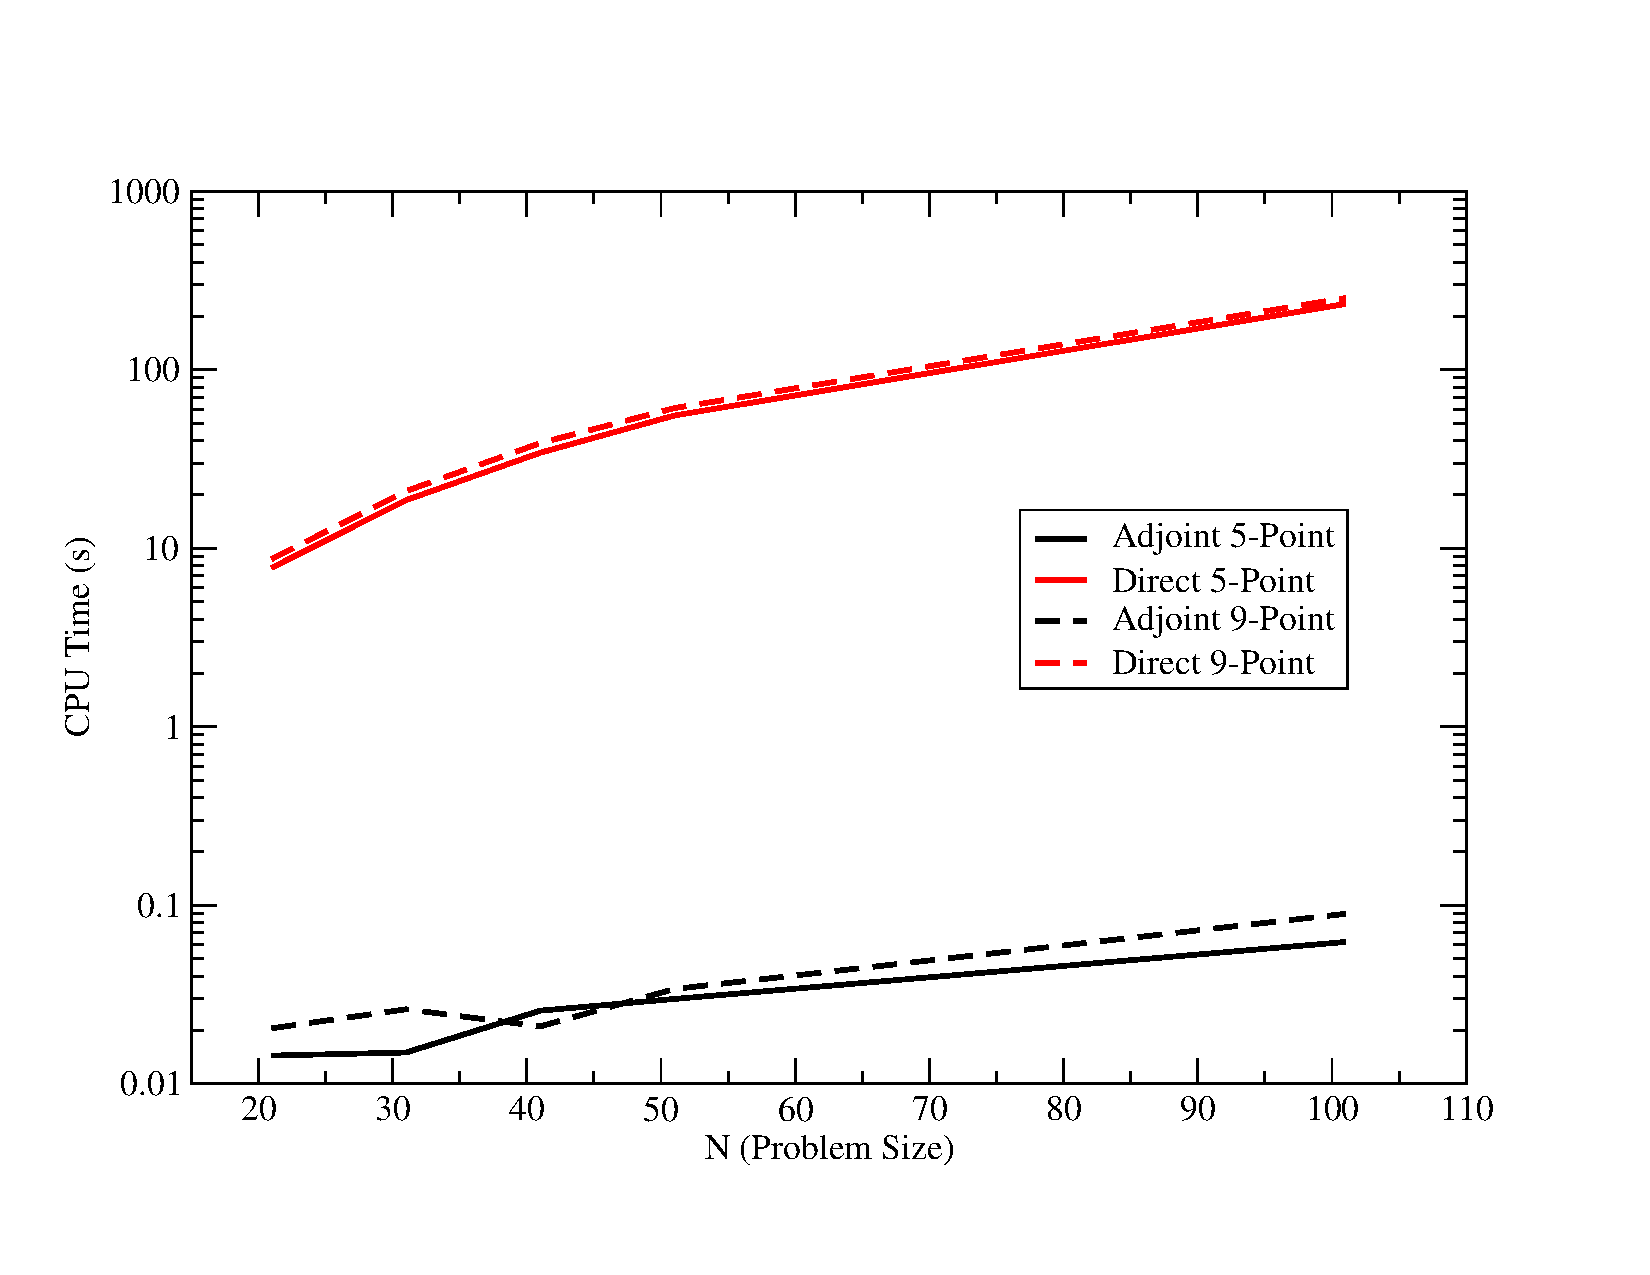
\includegraphics[width=5in,clip]{chapters/research_proposal/Adjoint_Direct_CPU_Time.pdf}
  \caption{\textbf{CPU Time (s) to converge vs. Problem Size ($N$ for
      an $N \times N$ square mesh).} \textit{Both the adjoint and
      direct solvers are used with the five point and nine point
      stencils. A significant CPU time speedup is noted with the
      adjoint method due to the reduced number of random walk
      events.}}
  \label{fig:poisson_cpu_time}
\end{figure}

\begin{figure}[h!]
  \centering
  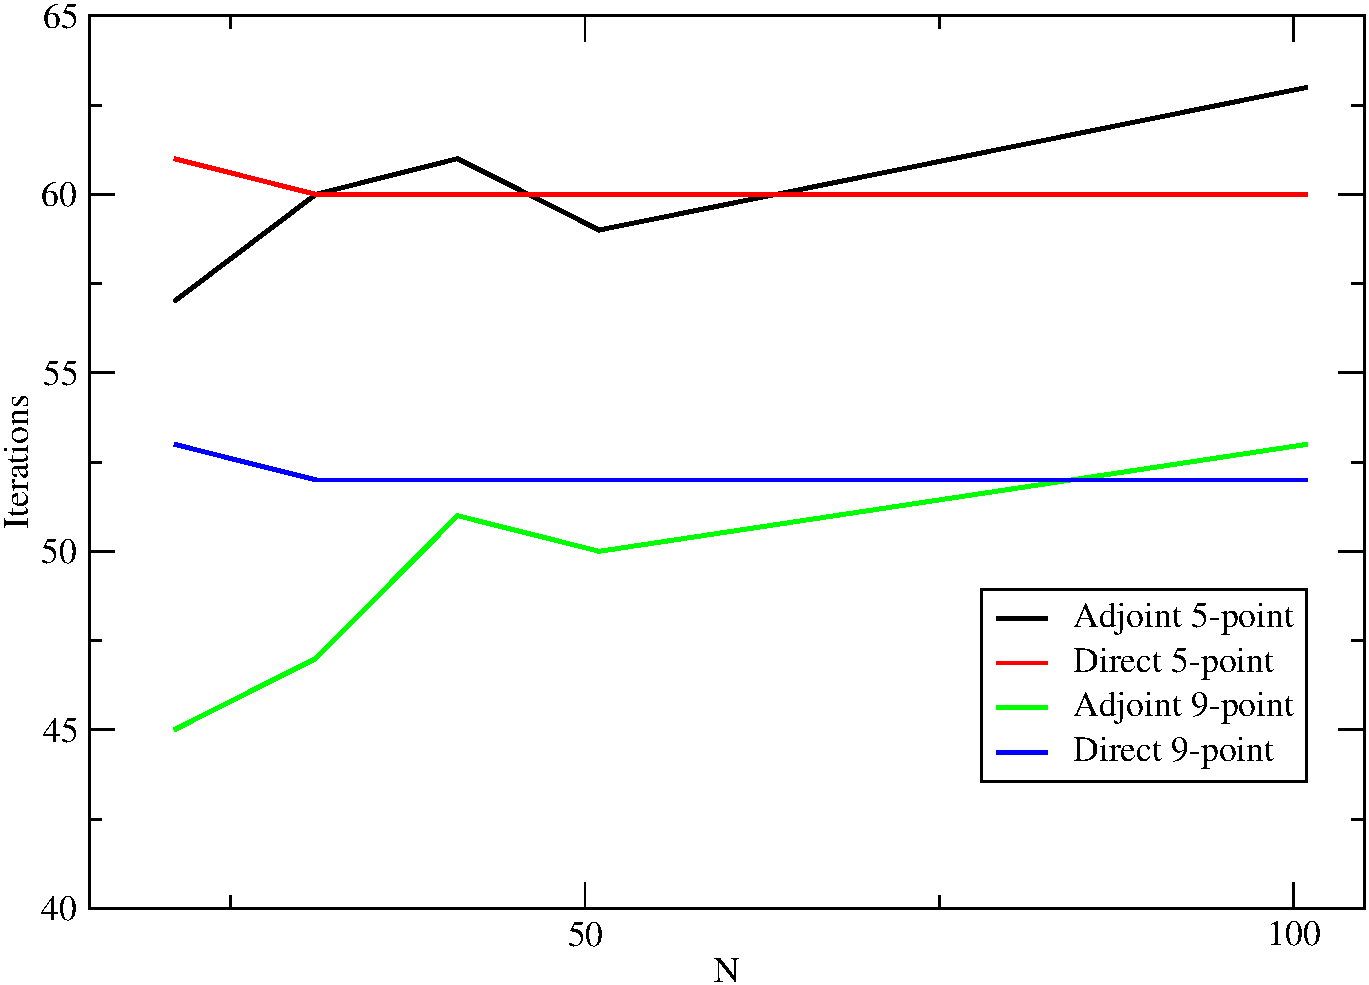
\includegraphics[width=5in,clip]{chapters/research_proposal/Adjoint_Direct_Iterations.pdf}
  \caption{\textbf{Iterations to converge vs. Problem Size ($N$ for an
      $N \times N$ square mesh).} \textit{Both the adjoint and direct
      solvers are used with the five-point and nine-point
      stencils. Both methods give similar iteration behavior.}}
  \label{fig:poisson_iterations}
\end{figure}

We see clearly in Fig.~\ref{fig:poisson_cpu_time} that the using the
adjoint solver with MCSA results in several orders of magnitude
speedup over the direct solver while the number of iterations required
to converge is of a similar scale. We expect this for several
reasons. First, with an equivalent number of histories specified for
both solvers and a system of size $N \times N$, the direct solver will
compute $N \times N$ random walks per permutation while the adjoint
solver will only compute one. This is necessary in the direct method
to ensure a contribution from each state as the random walk sequence
will only contribute to the starting state. For the adjoint method,
because the random walk sequence contributes to the state in which it
currently resides, fewer histories are necessary to compute
contributions from all the nonzero parts of the source. Initially,
this may not seem like a fair comparison; however, we see from
Fig.~\ref{fig:poisson_iterations} that the number of iterations
required to converge is approximately the same and therefore the extra
computations performed by the direct method do not improve the error
estimation. Therefore, although the total number of random walks per
iteration is in fact larger for the direct method, the solution
computed at each iteration is no better than that computed by the
adjoint method.

As an additional comparison, the convergence behavior of MCSA can be
analyzed using both solvers to detect any performance benefits. To
assess the convergence properties of MCSA using each solver and
stencil, the infinity norm of the residual computed in
Eq.~(\ref{eq:mcsa}) was collected at each iteration for a fixed
problem size. Figure~\ref{fig:poisson_convergence} gives the results
of these computations. First, it is worthy to note on the semi-log plot
that we are indeed achieving the expected exponential convergence from
MCSA. Second, we note that both the direct and adjoint methods have
approximately equivalent convergence behavior, leading to CPU time
being the dominating factor in method selection.
\begin{figure}[h!]
  \centering
  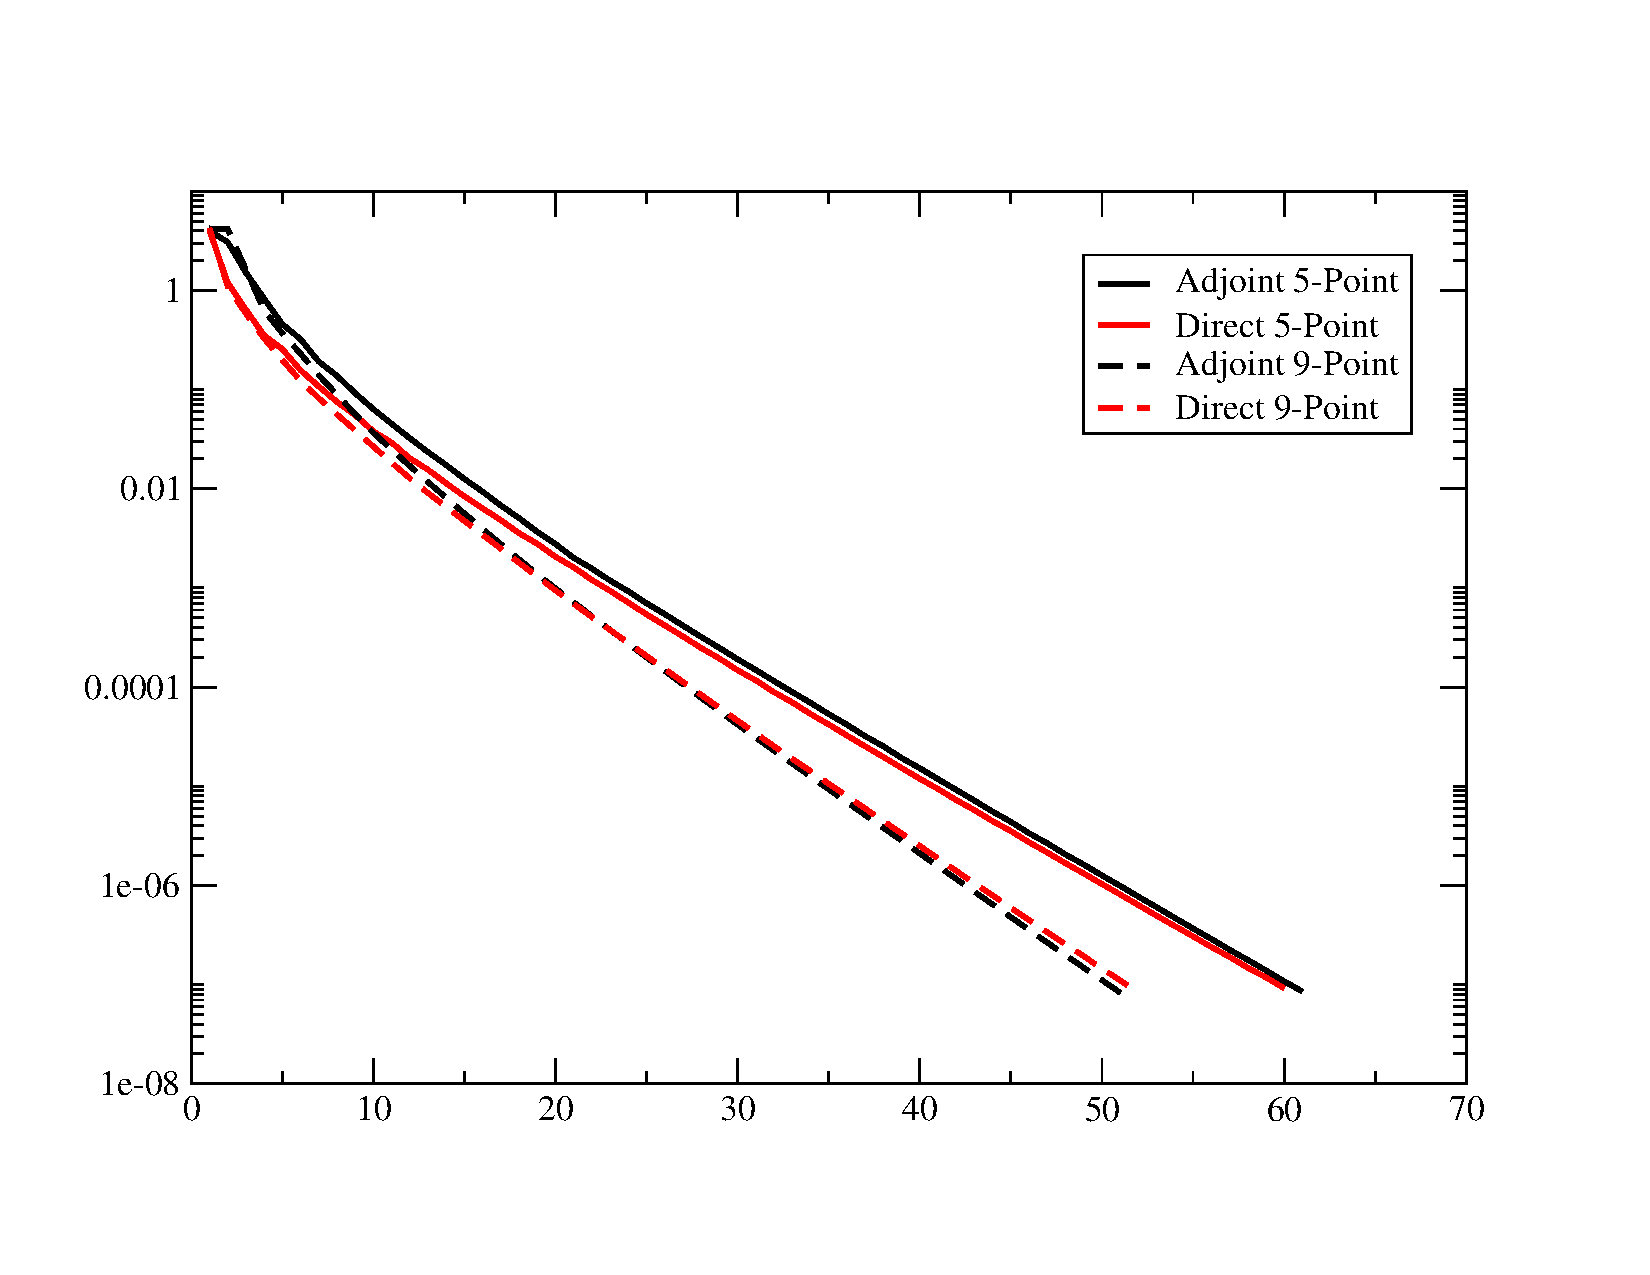
\includegraphics[width=5in,clip]{chapters/research_proposal/Adjoint_Direct_Convergence.pdf}
  \caption{\textbf{Infinity norm of the solution residual
      vs. iteration number for a problem of fixed size.} \textit{Both
      the adjoint and direct solvers are used with the five point and
      nine point stencils.}}
  \label{fig:poisson_convergence}
\end{figure}

\subsection{MCSA Application to Finite Element Problems}
\label{subsec:mcsa_finite_element}
The Epetra-based MCSA implementation has enabled the solution of
finite element problems leveraging the Panzer finite element assembly
engine, providing an initial basis for our experimental framework. To
demonstrate this, consider the 2-dimensional steady-state heat
equation:
\begin{equation}
  \boldsymbol{\nabla} \cdot k \boldsymbol{\nabla} T = Q\:,
  \label{eq:heat_equation}
\end{equation}
where $k$ is the thermal conductivity, $T$ is the temperature, and $Q$
is the thermal source. We can write the heat equation in weak form
using Eq~(\ref{eq:fe_weak_form}):
\begin{equation}
  \int_{\Omega} \boldsymbol{\nabla}^T \ve{v} k \boldsymbol{\nabla} T
  d\Omega - \int_{\Omega} \ve{v}Q d\Omega - \int_{\Gamma} \ve{v}
  \bar{q} d\Gamma - \int_{\Gamma} \ve{v} k \frac{\partial T}{\partial
    n} d\Gamma= 0\:,
  \label{eq:weak_heat_equation}
\end{equation}
where the boundary conditions have now been incorporated. We can
interpret the last two integral terms as the contributions from a
fixed boundary flux source and the flux through the domain
boundary. This weak formulation can then be directly implemented
within the finite element assembly engine along with the appropriate
boundary conditions and source terms. For this example, we choose a
square Cartesian grid with boundary conditions as shown in
Figure~\ref{fig:heat_eq_setup}.  
\begin{figure}[htpb!]
  \begin{center}
    \scalebox{1.5}{
      \input{chapters/research_proposal/heat_eq_setup.pdftex_t} }
  \end{center}
  \caption{\textbf{Problem setup for finite element solution to 2D
      heat equation.} \textit{Dirichlet conditions are set for the
      temperature on all 4 boundaries of the Cartesian grid with
      thermal conductivity set to 2.0. No thermal source was
      present.}}
  \label{fig:heat_eq_setup}
\end{figure}
A value of 2.0 is used for $k$ with no thermal source and second-order
basis functions are chosen for the finite element form. This problem
was solved using Panzer to assemble the finite element system and
Jacobi preconditioned MCSA as the linear solver with the adjoint
Neumann-Ulam method as the Monte Carlo solver. The results of this
calculation are presented in Figure~\ref{fig:heat_eq_solution}.
\begin{figure}[htpb!]
  \centering
  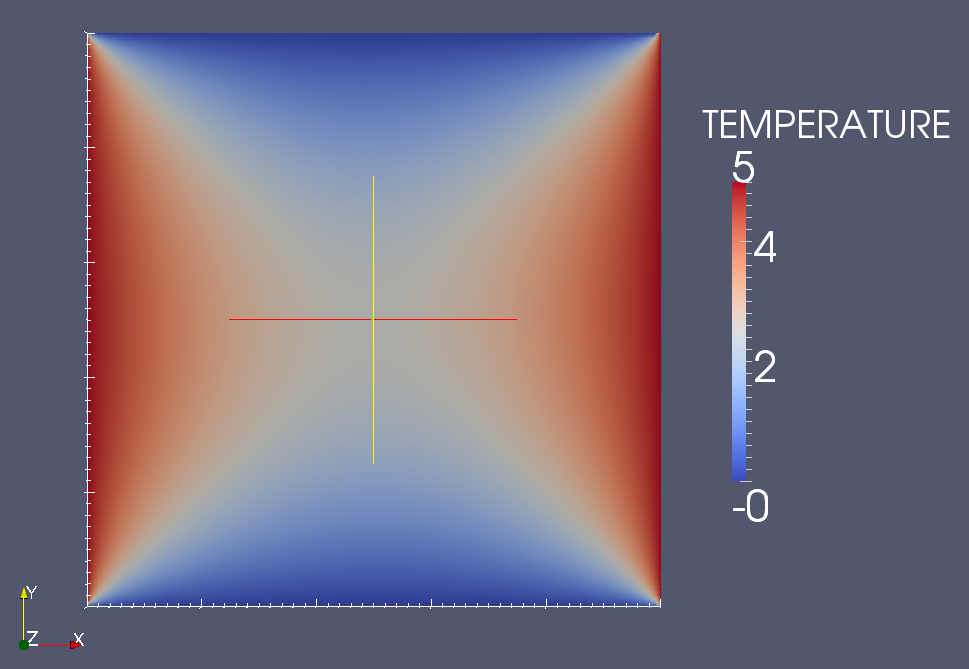
\includegraphics[width=5in,clip]{chapters/research_proposal/heat_eq_solution.png}
  \caption{\textbf{Finite element solution to the 2D steady-state heat
      equation using MCSA.} \textit{A $100 \times 100$ Cartesian grid
      was used with Jacobi preconditioning applied to the linear
      system.}}
  \label{fig:heat_eq_solution}
\end{figure}
In the results, we see the characteristic parabolic solution profiles
of the heat equation corresponding to the correct Dirichlet
condition. Based on this work, a finite element formulation generated
by the Panzer framework can be readily solved with a general MCSA
implementation. In addition, the above problem can already be solved
in parallel with conventional Krylov methods. Therefore, once a
parallel MCSA implementation is complete, this framework can be used
to generate those experiments and immediately compare to Krylov
methods. In addition, extension to nonlinear model problems requires
only a few small additions to the framework, providing the remainder
of the tool set we need for our analysis.

\section{Monte Carlo Methods Verification}
\label{sec:method_verification}
As we perform our numerical experiments, the results from the new
tools that we are using must be verified against benchmark
results. These benchmark tests should allow use to verify that the new
stochastic solvers that we develop generate the expected numerical
results in parallel for linear and nonlinear problems that have a
known, well-documented solution. In addition, as we explore parallel
strategies for the Monte Carlo methods and introduce bias or
non-reproducible results into our solution estimators, these
verification problems will allow us to determine if that cost is
acceptable. To verify the linear solvers, we will choose the above
2-dimensional heat equation problem in Eq~(\ref{eq:heat_equation}) on
a rectilinear grid for which analytical solutions are available. As a
complement to comparison with the analytical solutions, we may also
check those results against production implementations of Krylov
solvers. For the nonlinear solvers, we employ a new set of equations
with readily available benchmark solutions. In both cases, we
verification will be determined by comparing the locations of global
minima and maxima in the solution as well as comparison of solution
vector norms with respect to a specified tolerance.

\subsection{FANM Verification}
\label{subsec:fanm_verification}
To verify the FANM method for nonlinear problems, we choose benchmark
solutions for the 2-dimensional, steady, incompressible Navier-Stokes
equations on a rectilinear grid in much the same way as Shadid and
Pawlowski's work on Newton-Krylov methods for the solution of these
equations \citep{shadid_inexact_1997,pawlowski_globalization_2006}. We
define these equations as follows:
\begin{subequations}
  \begin{gather}
    \rho \ve{u} \cdot \nabla \ve{u} - \nabla \cdot \ve{T} - \rho
    \ve{g} = \ve{0}
    \label{eq:ns_momentum}\\
    \nabla \cdot \ve{u} = 0
    \label{eq:ns_continuity}\\
    \rho C_p \ve{u} \cdot \nabla T + \nabla \cdot \ve{q} = 0\:,
    \label{eq:ns_energy}
  \end{gather}
  \label{eq:navier_stokes}
\end{subequations}
where $\rho$ is the fluid density, $\ve{u}$ is the fluid velocity,
$\ve{g}$ gravity, $C_p$ the specific heat capacity at constant
pressure of the fluid and $T$ the temperature of the
fluid. Eq~(\ref{eq:ns_momentum}) provides momentum transport,
Eq~(\ref{eq:ns_continuity}) provides the mass balance, and
Eq~(\ref{eq:ns_energy}) provides energy transport with viscous
dissipation effects neglected. In addition, we close the system with
the following equations:
\begin{subequations}
  \begin{gather}
    \ve{T} = -P \ve{I} + \mu[\nabla \ve{u} + \nabla \ve{u}^T]
    \label{eq:ns_stress_tensor}\\
    \ve{q} = - k \nabla T\:,
    \label{eq:ns_heat_flux}
  \end{gather}
  \label{eq:ns_closure}
\end{subequations}
where $\ve{T}$ is the stress tensor, $P$ is the hydrodynamic pressure,
$\mu$ is the dynamic viscosity of the fluid, $\ve{q}$ is the heat flux
in the fluid, and $k$ is the thermal conductivity of the fluid. This
set of strongly coupled equations possesses both the nonlinearities
and asymmetries that we are seeking for qualification of the FANM
method. Further, physical parameters within these equations can be
tuned to enhance the nonlinearities. We will then apply these
equations to the following three standard benchmark problems.

\subsubsection{Thermal Convection Cavity Problem}
\label{subsubsec:natural_convection_cavity}
In 1983 a benchmark solution for the natural convection of air in a
square cavity was published \citep{de_vahl_davis_natural_1983} as
shown in Figure~\ref{fig:natural_convection_cavity} for the solution
of the energy, mass, and momentum equations.
\begin{figure}[htpb!]
  \begin{center}
    \scalebox{1.5}{
      \input{chapters/research_proposal/natural_convection_cavity.pdftex_t} }
  \end{center}
  \caption{\textbf{Problem setup for the natural convection cavity
      benchmark.} \textit{Dirichlet conditions are set for the
      temperature on the left and right while Neumann conditions are
      set on the top and bottom of the Cartesian grid. The temperature
      gradients will cause buoyancy-driven flow. Zero velocity
      Dirichlet conditions are set on each boundary. No thermal source
      was present.}}
  \label{fig:natural_convection_cavity}
\end{figure}
In this problem, a rectilinear grid is applied to the unit square. No
heat flow is allowed out of the top and bottom of the square with a
zero Neumann condition specified. Buoyancy driven flow is generated by
the temperature gradient from the cold and hot Dirichlet conditions on
the left and right boundaries of the box. By adjusting the Rayleigh
number of the fluid (and therefore adjusting the ratio of convective
to conductive heat transfer), we can adjust the influence of the
nonlinear convection term in Eq~(\ref{eq:ns_momentum}). In Shadid's
work, Rayleigh numbers of up to \sn{1}{6} were used for this benchmark
on a $100 \times 100$ square mesh grid.

\subsubsection{Lid Driven Cavity Problem}
\label{subsubsec:lid_driven_cavity}
As an extension of the convection problem, the second benchmark
problem given by Ghia \citep{ghia_high-re_1982} adds a driver for the
flow to introduce higher Reynolds numbers into the system, providing
more inertial force to overcome the viscous forces in the fluid. The
setup for this problem is equally simple, containing only the
Dirichlet conditions as given in Figure~\ref{fig:lid_driven_cavity}
and is only applied to the mass and momentum equations on the unit
square.
\begin{figure}[htpb!]
  \begin{center}
    \scalebox{1.5}{
      \input{chapters/research_proposal/lid_driven_cavity.pdftex_t} }
  \end{center}
  \caption{\textbf{Problem setup for the lid driven cavity benchmark.}
    \textit{Dirichlet conditions of zero are set for the velocity on
      the left and right and bottom while the Dirichlet condition set
      on the top provides a driving force on the fluid.}}
  \label{fig:lid_driven_cavity}
\end{figure}
The top boundary condition will provide a driver for the flow and its
variation will in turn vary the Reynolds number of the fluid. An
increased velocity will generate more inertial forces in the fluid,
which will overcome the viscous forces and again increase the
influence of the nonlinear terms in Eq~(\ref{eq:ns_momentum}). Shadid
also used a $100 \times 100$ grid for this benchmark problem with
Reynolds numbers up to \sn{1}{4}.

\subsubsection{Backward-Facing Step Problem}
\label{subsubsec:backward_facing_step}
The third benchmark was generated by Gartling in 1990 and consists of
both flow over a backward step and an outflow boundary condition
\citep{gartling_test_1990}. Using the mass and momentum equations
while neglecting the energy equation, this problem utilizes a longer
domain with a 1/30 aspect ratio with the boundary conditions as shown
in Figure~\ref{fig:backward_facing_step}.
\begin{figure}[htpb!]
  \begin{center}
    \scalebox{1.3}{
      \input{chapters/research_proposal/backward_facing_step.pdftex_t} }
  \end{center}
  \caption{\textbf{Problem setup for the backward facing step
      benchmark.} \textit{Zero velocity boundary conditions are
      applied at the top and bottom of the domain while the outflow
      boundary condition on the right boundary is represented by zero
      stress tensor components in the direction of the flow. For the
      inlet conditions, the left boundary is split such that the top
      half has a fully formed parabolic flow profile and the bottom
      half has a zero velocity condition, simulating flow over a
      step.}}
  \label{fig:backward_facing_step}
\end{figure}
In this problem, the inflow condition is specified by a fully-formed
parabolic flow profile over a zero velocity boundary representing a
step. The flow over this step will generate a recirculating backflow
under the inlet flow towards the step. As in the lid driven cavity
problem, the nonlinear behavior of this benchmark and the difficulty
in obtaining a solution is dictated by the Reynolds number of the
fluid. In Shadid's work, a $20 \times 400$ non-square rectilinear grid
was used to discretize the domain with Reynolds number up to
\sn{5}{2}.

\section{Proposed Numerical Experiments}
\label{sec:numerical_experiments}
Using the verification problems for the linear and nonlinear solvers
as a testing environment, we propose a set of experiments that will be
used to characterize several qualities of parallel Monte Carlo
solvers. At the end of Chapter~\ref{ch:stochastic_methods}, we posed
several research questions related to the parallelization of the
adjoint Neumann-Ulam method and the MCSA method while in
Chapter~\ref{ch:nonlinear_problem} we posed questions related to the
FANM method. We will generate numerical experiments from these
questions by dividing them into 4 categories: domain overlap studies
for the parallel Neumann-Ulam method, domain replication studies for
the parallel Neumann-Ulam method, parallel performance and numerical
accuracy studies for the MCSA method, and parallel performance and
numerical accuracy studies for the FANM method.

\subsection{Domain Overlap Studies for the Parallel Neumann-Ulam
  Method}
\label{subsec:domain_overlap_studies}
Characterizing and understanding the domain overlap behavior of a
parallel Neumann-Ulam method will be critical to efficient
implementations of other solvers that will be built on top of these
methods. In the reactor physics work that we reviewed, the amount
domain overlap used could be directly correlated to physical
parameters of the system, namely the dimension of repeated geometric
structures and the mean free path of neutrons in the system. We
therefore seek analogous measurements for the general linear
system. These measurements will characterize how far from its starting
state a random walk sequence moves as a function of properties of the
linear system. Our experimental framework will allow us to fix various
properties of the system while varying others including the size of
the linear system, its spectral radius, its sparsity, its asymmetry,
and other parameters related to the Eigenvalues, conditioning, and
structure of the linear operator. By varying the domain overlap and
measuring parallel performance with respect to these properties, we
can develop guidelines for setting the overlap with respect to
measurable properties of the linear operator. In addition, varying the
amount of overlap will allow us to measure the additional memory costs
incurred.

\subsection{Domain Replication Studies for the Parallel Neumann-Ulam
  Method}
\label{subsec:domain_replication_studies}
Employing domain replication with the Neumann-Ulam method will be an
exercise in batch statistics. By using replication, we also expect to
incur an additional memory overhead. As noted in previous work, domain
replication was coupled with domain overlap in order to improve load
balancing and scalability in the implementations. As replication will
likely be required to solve future resiliency issues and may even by
required by this work in order to achieve scalability, its parallel
performance must also be measured. We will therefore measure the
memory and performance overhead incurred by varying the amount of
domain replication leveraged by the Neumann-Ulam solver with respect
to a fixed linear system.

\subsection{Parallel Performance and Numerical Accuracy Studies for
  the MCSA Method}
\label{subsec:mcsa_studies}
A parallel MCSA implementation and our numerical test framework will
allow us to compare its performance to Krylov methods and allow us to
experiment with the way we combine it with the Neumann-Ulam solver. As
discussed in \S~\ref{subsec:parallel_adjoint}, previous work with MCSA
used a correction generated by the Neumann-Ulam method with a fairly
large uncertainty near 14\%. We hypothesized that if we can identify
the amount of overlap in our Neumann-Ulam experiments required to
eliminate most transitions between adjacent domains owned by different
processors, then perhaps transport to adjacent domains can be
ignored. This will result in a biased estimator for the MCSA
correction that cannot be reproduced, however, these studies will aim
to determine if that bias and lack of reproducibility affects the
numerical results and reproducibility of the MCSA method, yielding a
critical outcome for this work. Furthermore, we will use the
experimental framework to measure the convergence rates for
non-symmetric systems and memory usage of the MCSA algorithm and
compare them to conventional Krylov methods using the same framework.

\subsection{Parallel Performance and Numerical Accuracy Studies for
  the FANM Method}
\label{subsec:fanm_studies}
Aside from resiliency motivations, the primary driver behind the FANM
method is reduced memory pressure due to the lack of additional
storage beyond that of the linear system in the MCSA method. The
nonlinear benchmark problems we have chosen will let us measure this
memory usage and compare it to conventional Newton-Krylov
methods. Furthermore, by varying the strength of the nonlinearities in
those problems (effectively by increasing the amount of convective
transport in the system), the benchmarks will become more difficult to
solve and require even more iterations to converge. This will give us
a means by which to vary the complexity of the system which we can
then compare to memory usage. Additionally, with the finite element
assembly framework we can choose functional discretizations of varying
accuracy, allowing us to vary the degrees of freedom in the system and
therefore also vary the memory required for each problem.

\section{Proposed Challenge Problem}
\label{sec:challenge_problem}
Our numerical experiments will provide us with a set of metrics giving
best-performance Monte Carlo solver parameters for problems of
different types. As an additional bonus, these experiments will let us
further develop new parallel implementations of the Monte Carlo methods
in order to improve their performance and scalability. With these
advancements in hand, we look forward towards applying them to
large-scale problems in reactor physics. The Consortium for Advanced
Simulation of Light Water Reactors (CASL) is a Department of Energy
Modeling and Simulation Hub focused on predictive multiphysics
modeling of nuclear reactors
\citep{u.s._department_of_energy_casl_2011}. Their efforts are focused
on enabling nuclear reactor analysis and development using today's
supercomputing technology to achieve higher power uprates, higher fuel
burn-up, and predictive accident scenario analysis. As a means of
driving their research and development, CASL has worked with the
nuclear industry to identify challenge problems of critical importance
to achieving these goals.

To meet some of the high fidelity modeling requirements of these
challenge problems, the Drekar multiphysics code is being developed at
Sandia National Laboratories for fluid flow and conjugate heat
transfer problems \citep{pawlowski_drekar_2012}. Drekar is being
used to analyze complex problems including the grid-to-rod-fretting
(GTRF) phenomena observed in light water reactor fuel rods. GTRF
occurs due to the turbulent flow of water through the subchannels of
the reactor core. This turbulence causes the nuclear fuel pins to
vibrate and the fuel cladding to wear against structures in the
reactor, causing localized hot spots and ultimately cladding
failure. Reducing these instances of failure and understanding how
they occur through predictive multiple physics simulation of fluid
flow and heat transfer will permit more robust fuel assembly
designs. In addition, the turbulence studies that Drekar performs will
allow for improved flow patterns to be generated in the assembly
subchannels, allowing for better heat transfer between the nuclear
fuel and the water, ultimately allowing for a more efficient reactor.

Drekar is a massively parallel physics framework built upon the same
Panzer library as well as other open-source tools that we are
leveraging in our own experimental framework. Furthermore, its
multiphysics formulation utilizes Newton-Krylov methods to generate a
fully consistent solution scheme for the Navier-Stokes equations with
various turbulence models for fluid simulation as well as the heat
conduction problem for simulation in solid materials. Performance
metrics show scaling to $O(100,000)$ cores on leadership class
machines with $O(\sn{1}{9})$ degrees of freedom in these
simulations. Given these features, Drekar will be an excellent
framework in which we can pose our own challenge problem for the FANM
and newly parallelized MCSA methods proposed by this research. At the
time our preliminary numerical experiments are completed for
characterizing the parallel FANM and MCSA implementations, we propose
implementing them within the Drekar framework and performing the
equivalent of its largest GTRF multiphysics problem to date, most
likely to be a fuel-assembly sized problem. Doing so will allow us to
not only implement our new methods in a production physics code and
apply it to a problem of great interest to the nuclear community, but
it will also allow us to compare its performance and scaling to the
Newton-Krylov methods currently leveraged within Drekar. If
successful, we expect to demonstrate improved computational
performance from a memory usage and/or an algorithmic scaling
perspective.

\section{Conclusion}
\label{sec:conclusion}
We have proposed the research and development of novel, massively
parallel Monte Carlo methods for the solution of linear and nonlinear
problems. These new methods aim to enhance the solution of multiple
physics problems of great national interest. Current progress has
shown that these methods can indeed be expanded into a general linear
algebra framework that permits their application to a broad range of
problems. Additional analysis has also been completed that begins to
characterize their performance in different configurations. Leveraging
this work, we have defined a multiphysics framework based on the
finite element method and have demonstrated that these Monte Carlo
methods can be used effectively to solve the linear systems generated
by these discretizations.

To guide our development of parallel Monte Carlo methods, we have
devised several classes of numerical experiments using our
multiphysics framework that will provide insight into their properties
and performance for linear and nonlinear problems. Furthermore, these
experiments aim to provide metrics that will give an indication of
both solver performance for various problem types and the type of
parallel decomposition required to effectively solve these
problems. Domain decomposition, domain replication, and their
combination will be of great interest for the analysis of parallel
Monte Carlo methods while algorithm scalability and memory usage will
be of interest for the MCSA and FANM methods that leverage them.

We culminate our research and development with a challenge problem by
applying these new Monte Carlo methods in the Drekar multiphysics
code. With Drekar, we look forward to providing a new and robust
solution method at the production scale. Using these tools and a
leadership class computing platform, we will provide performance
measurements for the Monte Carlo solvers and compare them to
conventional methods currently leveraged within Drekar. Given the
potential to improve computational performance in production
environments such as Drekar, these new methods have the potential to
help meet the high fidelity modeling and simulation needs of the
nuclear community.
